\newcommand{\checkbox}[1]{\raisebox{-.15em}{\Square}\ \textbf{#1} \\}

\addchap{Erstsemester-Checkliste}

Für einen erfolgreichen Start in das Studium solltest du einige organisatorische Kleinigkeiten unbedingt in den ersten Wochen erledigen.
Diese haben wir dir in folgender Checkliste mit absteigender Priorität zusammengestellt.

\checkbox{Wohnung}
Solltest du noch keine Bleibe gefunden haben, ist Beeilung angesagt, die schönsten Wohnungen sind schnell weg.
Wenn du in den Genuss eines 10- bzw. 100-Mbit/s-Internetzugangs kommen möchtest, seien dir die Wohnheime \link{http://www.studentenwerk-dresden.de/wohnen/wohnheimkatalog} des Studentenwerks Dresden empfohlen. Alternativ bieten sich auch Portale wie \textit{WG-Gesucht} \link{http://wg-gesucht.de/} an.

\checkbox{Studienrelevante Dokumente}
Das Vorlesungsverzeichnis und die Prüfungs- und Studienordnung erhälst du direkt beim Prüfungsamt \link{http://tu-dresden.de/inf/pra}.
Gedruckte Ordnungen gibts beim FSR und in deiner ESE-Tüte.
Alle wichtigen Informationen zu den einzelnen Vorlesungen findest du auf den jeweiligen Seiten der Institute im Netz.
Die Professoren werden dir dazu jedoch auch noch alles in den ersten Vorlesungen mitteilen. Sonst hilft natürlich schon einmal ein Blick auf die Seite des FSR \link{http://www.ifsr.de}.

\checkbox{Mail Account}
Siehe \textit{ZIH} in diesem Heft. Wichtig ist vor allem auch, das Erstpasswort zu ändern. Besuche hierfür am besten den Identity Manager des ZIH \link{https://idm-service.tu-dresden.de}.

\checkbox{E-Meal Karte}
Die Mensa Karte gibt es während der ESE oder in den Mensen selbst für jeweils 5\euro\ Pfand.
Zusätzlich dazu benötigst du eine E-Meal Bescheinigung, die du auf deinem Semesterbogen findest.

\checkbox{(optional) Sprachkurse}
Die TU bietet Sprachkurse für Englisch und viele weitere Sprachen an. Zur Einschreibung in den Informatik Master (nach dem Bachelor) müssen Englischkenntnisse nachgewiesen werden. Die Einschreibung für die Sprachkurse wird je nach Kurs im Laufe der ersten beiden Wochen deines Studiums freigeschaltet.
Erkundige dich auf den Seiten des LSK \link{https://lskonline.tu-dresden.de} frühzeitig, wann dies ist. Die meisten Kurse sind sehr schnell voll.

\checkbox{(optional) Sportkurse}
Wie für die Sprachkurse gilt auch hier, wer zuerst da ist...
Das Angebot kannst du beim Universitätssportzentrum (USZ) einsehen \link{http://tu-dresden.de/die_tu_dresden/zentrale_einrichtungen/usz}.
Hast du dich für einen Kurs entschieden und bei freigeschalteter Einschreibung für diesen angemeldet, musst du nur noch die Anmeldebescheinigung drucken und den Kostenbeitrag innerhalb von drei Tagen auf das Konto des USZ überweisen.

\checkbox{Wohnsitz anmelden}
Offiziell musst du innerhalb von zwei Wochen beim zuständigen Ortsamt \link{http://www.dresden.de/de/02/or/anliegen/c_233.php} deine Wohnung anmelden.
Wer seinen Hauptwohnsitz nach Dresden verlegt bekommt von der Stadt eine "Umzugsbeihilfe" in Höhe von 150\euro.
Informationen dazu gibt's unter \link{http://www.dresden.de/de/02/or/anliegen/c_336.php} und \link{http://www.studentenwerk-dresden.de/wohnen/umzugsbeihilfe.html}.
Wenn die Wohnung als Nebenwohnsitz anmeldet wird, muss Zweitwohnsteuer gezahlt werden. Diese beträgt 10\% der Kaltmiete pro Monat. Weitere Informationen findest du beim StuRa \link{www.stura.tu-dresden.de/zweitwohnungssteuer}.

\checkbox{BAföG Antrag}
Formulare und Auskunft gibt es beim Studentenwerk (4. Etage).
Schiebe den Antrag nicht allzu lang vor dir her, da dein Anspruch für abgelaufene Monate verfällt.
Informationen zu den Sprechzeiten beim Studentenwerk gibt es hier \link{http://www.studentenwerk-dresden.de/finanzierung/servicebuero.html}.

\checkbox{Bibliotheksausweis}
Bekommt man direkt am Schalter in der SLUB (Zellescher Weg 18) \link{http://www.slub-dresden.de/service/anmelden}.

\checkbox{Copycard}
Drucker der Firma Ricoh stehen quer über den Campus verteilt und lassen sich von jedem Rechner mit einer Copycard ansprechen.
Diese bekommst du in der StuRa Baracke hinter dem Hörsaalzentrum für 5\euro\ Pfand. Du kannst aber auch direkt beim FSR für geringe Kosten drucken (einfach Dokumente per USB Stick mitbringen).

\checkbox{C und Java-Kurs}
Besonders denjenigen ohne Programmiererfahrung werden die im Wintersemester angebotenen C und Java-Kurse ans Herz gelegt.
Diese finden in der Regel unter der Woche statt, manche auch am Wochenende.
Für Details wendet euch an \link{programmierung@ifsr.de}, \link{fredo@ifsr.de} und behaltet die News auf \link{https://www.ifsr.de} im Auge.

\checkbox{Fachschaftsratwahlen}
Wähle deine studentischen Vertreter im FSR Informatik.
Die Wahlen finden jedes Jahr im November statt.
Geh wählen!
Und noch besser: Lass dich wählen!

\checkbox{Prüfungseinschreibung}
Ab Ende Januar kann man sich in jExam zu den Prüfungen anmelden.
Schreib dich in die Prüfungen der Fächer ein, die du besucht hast.
Viel Erfolg!

\checkbox{Rückmeldung zum Sommersemester}
Ab Mitte Januar 2015 kannst du den Semesterbeitrag für das nächste Semester überweisen.
Den genauen Betrag und Termine findest du auf dem aktuellen Semesterbogen und hier \link{http://tu-dresden.de/studium/organisation/rueckmeldung/semesterrueckmeldung}.
Kümmere dich rechtzeitig darum, sonst wirst du automatisch exmatrikuliert!

\vfill

\begin{figure}[h!]
\centering
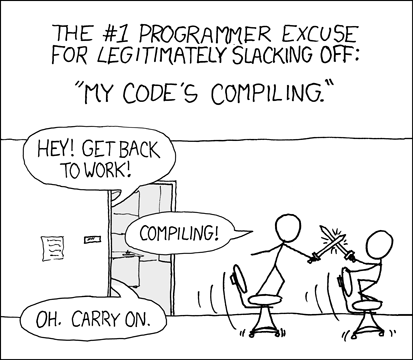
\includegraphics[scale=.5]{img/xkcd/compiling.png}
\caption*{{\small \textit{'Are you stealing those LCDs?' 'Yeah, but I'm doing it while my code compiles.' (xkcd.com/303)}}}
\end{figure}
